\documentclass[12pt,twoside]{article} 

\usepackage[hmarginratio=1:1]{geometry}

\usepackage{graphicx}
\usepackage[utf8]{inputenc}
%\usepackage{amsmath}
\usepackage{fancyhdr}


\title{Diseño y construcción de un sistema UAV}
\author{Jordi Pérez Talamino \and Jordi Rebull Mestres}
\date{\today}

\begin{document}

\pagestyle{fancy}

\fancyhead{}

\fancyhead[RO,LE]{\thepage}
\fancyhead[RE,LO]{Quadcopter}

\fancyfoot{}
\fancyfoot[C]{
\includegraphics[scale=0.1]{Imatges/etseib.png}}
\maketitle

\newpage

\tableofcontents

\newpage
	
  \section{Introducción}\label{sec:intro}
	
		\subsection{Motivación Personal}\label{subsec:motiva}
		
		\subsection{Objetivos del proyecto}\label{subsec:objectivos}
		
\newpage

 \section{Estado del arte}\label{sec:estado arte}

		\subsection{Vehículos Aéreos no tripulados (UAV's)}\label{subsec:UAV}
		
		Un vehículo aéreo no tripulado (UAV: Unmanned Aerial Vehicle) es aquel que es capaz de navegar sin llevar a bordo ningún piloto, 
		controlándose a veces desde una estación base y con capacidad de navegar de forma autónoma mediante una programación preestablecida.
		Estos vehículos poseen muchas ventajas respecto a las aeronaves tripuladas para ciertas aplicaciones. Ya que con su uso no se ponen en riesgo vidas humanas, 
		destacan en el campo de reconocimiento del terreno y en la posibilidad de acceder a zonas peligrosas o de difícil acceso. 
		Por estos motivos, los UAV han sido utilizados sobretodo en aplicaciones militares, tales como el reconocimiento del terreno y el ataque a distancia.
			
			\subsubsection{Tipos}\label{subsubsec:Tipos UAV}
			
		\subsection{Cuadricópteros}\label{subsec:cuadricopteros}
		
		\subsection{Modelos Comerciales}\label{subsec:comerciales}
		
\newpage
\maketitle
	\section{Funcionamiento de un cuadricóptero}\label{sec:funcionamiento}
		Cualquier aeronave es capaz de realizar 3 posibles rotaciones alrededor de los 3 ejes de coordenadas con origen en el centro de gravedad de la aeronave. 
		Estos 3 ejes son: el eje lateral, el longitudinal y el vertical, y las maniobras se llaman cabeceo (en inglés, pitch), alabeo (roll) y guiñada (yaw), como se observa en la figura \ref{fig:rotations}.
		
		
		Un cuadricóptero se propulsa mediante cuatro conjuntos motor-hélice denominados rotores, situados en los extremos de la aeronave.
		Cada rotor en funcionamiento produce sobre la aeronave un empuje y un par sobre su eje de rotación. 
		Por este motivo, se utilizan 4 rotores idénticos y se colocan en forma de cruz (figura \ref{fig:quadrotorhover}), 
		donde dos de los rotores giran en un sentido, y los otros dos lo hacen en sentido opuesto.
		
		\begin{figure}
			\centering
			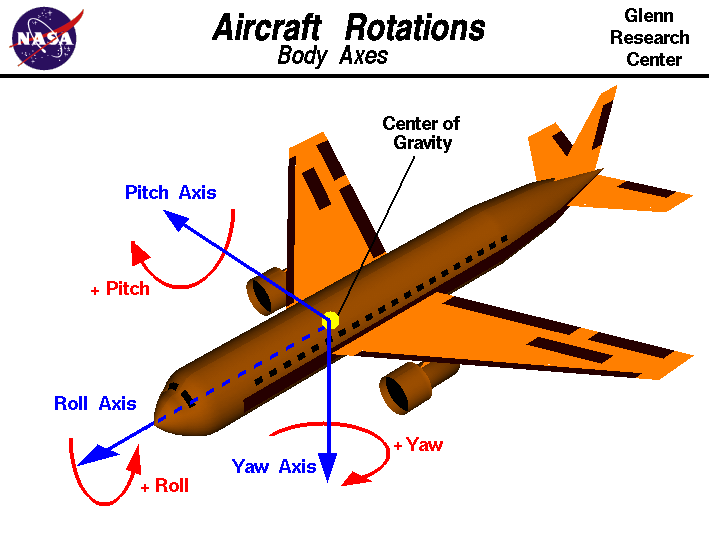
\includegraphics[width=0.9\textwidth]{Imatges/Funcionament/rotations.png}
			\caption{Rotaciones posibles}
			\label{fig:rotations}
		\end{figure}
		
		\begin{figure}
			\centering
			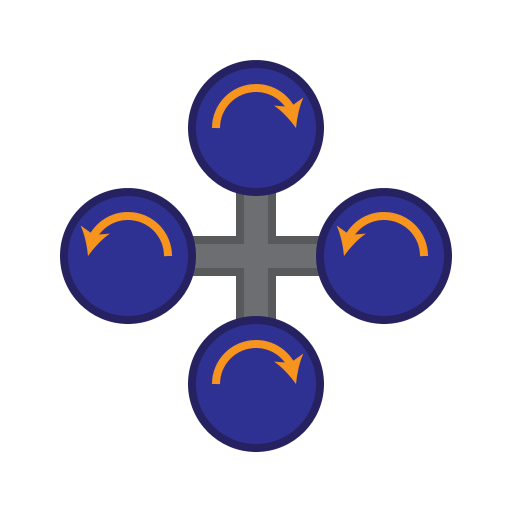
\includegraphics[width=0.5\textwidth]{Imatges/Funcionament/quadrotorhover.png}
			\caption{Distribución de los rotores en un cuadricóptero}
			\label{fig:quadrotorhover}
		\end{figure}
		
		Con esta configuración, si los 4 rotores giran con la misma velocidad angular, el par aerodinámico resultante sobre la aeronave es nulo, y entonces no hay aceleración angular en la dirección yaw. Así es como un quadricóptero se mantiene volando a una misma altitud y sin girar sobre si mismo, y acelerando o frenando por igual los 4 rotores es como gana o pierde altitud, respectivamente. 
		
		Para controlar el roll y el pitch, el cuadricóptero aumenta el empuje de un rotor y disminuye el empuje del rotor diametralmente opuesto (figura \ref{fig:quadrotorpitch_androll}).
		
		\begin{figure}
			\centering
			\includegraphics[width=0.5\textwidth]{Imatges/Funcionament/quadrotorpitch_androll.png}
			\caption{Control sobre el roll y el pitch}
			\label{fig:quadrotorpitch_androll}
		\end{figure}
		
		Para controlar el yaw, el cuadricóptero aumenta la velocidad de los dos motores que giran en un mismo sentido, y disminuye la velocidad de los otros dos (para no ganar ni perder altitud). De esta manera el par total resultante sobre la aeronave no se anula y se produce una rotación en el eje yaw (Figura \ref{fig:quadrotoryaw}).
		
		\begin{figure}
			\centering
			\includegraphics[width=0.5\textwidth]{Imatges/Funcionament/quadrotoryaw.png}
			\caption{Control sobre la rotación en el eje yaw}
			\label{fig:quadrotoryaw}
		\end{figure}
		
		Resumiendo estos conceptos, los 4 grados de libertad de control del cuadricóptero son:
		
		\begin{itemize}

			\item Acelerador (Throttle): acelera o frena los 4 rotores por igual
			\item Cabeceo (Pitch): gira la aeronave sobre su eje de cabeceo 
			\item Alabeo (Roll): gira la aeronave sobre su eje de alabeo
			\item	Guiñada (Yaw): gira la aeronave sobre su eje de guiñada

		\end{itemize}
		
		Mediante estos 4 movimientos y sus múltiples combinaciones se controla el movimiento del vehículo.

		\subsection{Chasis}\label{subsec:chasis}
		Como todo vehículo, el cuadricóptero necesita de un chasis o estructura. Sobre ella van colocados todos los componentes, y cumple tanto una función estructural como una función de protección de las partes más delicadas.
Es un elemento vital, porque según su diseño, tanto a nivel de geometría, como de qué materiales y uniones lo componen, afecta al comportamiento del vehículo. Además, el chasis debe ser capaz de aguantar las diferentes solicitaciones mecánicas que necesita la aeronave en sus distintas fases de operación, con la suficiente seguridad:

		\begin{itemize}

			\item Posado en tierra
			\item Despegues y aterrizajes (son siempre las maniobras más difíciles y peligrosas de cualquier aeronave)
			\item En vuelo
		\end{itemize}
		Ejemplos de estas fases son las vibraciones producidas durante el vuelo, debe tener una cierta rigidez, los contactos con el suelo durante el aterrizaje, etc.
Además, el chasis debe de tener los anclajes y soportes adecuados para los diferentes componentes que conforman el cuadricóptero, tanto los más vitales (por ejemplo los motores) como accesorios que deba llevar (equipos de video, fotografía...).


			
			
		\subsection{Sistema de propulsión}\label{subsec:propulsion}
		El sistema de propulsión está formado por 4 rotores idénticos. Cada rotor se compone de un motor que produce la energía mecánica necesaria para mover una hélice acoplada a él, la cual produce el empuje aerodinámico necesario para hacer volar la aeronave.
			\subsubsection{Motores}\label{subsubsec:motores}
			El cuadricóptero se alimenta de energía eléctrica proveniente de baterías, por lo cual se utilizan motores eléctricos para transformarla en la energía mecánica necesaria.
En el campo en el cual se enmarca el cuadricóptero (aeromodelismo y robótica), y dadas las dimensiones y peso necesario, las máquinas eléctricas más adecuadas y utilizadas son las siguientes:

		\begin{itemize}
			\item Máquina de corriente continua
			
			En este rango de tamaño y potencias reducidas, se compone de unos imanes permanentes en el estator (parte exterior fija) que crean un campo magnético constante y unas bobinas en el rotor (parte interior móvil) conectadas eléctricamente mediante escobillas.
			
El paso de corriente a través de las bobinas genera un 	campo magnético que 	reacciona con el campo magnético generado por los imanes, lo cual provoca un par de 	rotación y hace que el eje gire. Para mantener el giro indefinidamente, las bobinas 	están conectadas a una pieza llamada colector, de tal manera que van conmutando la 	polaridad al girar y se consigue crear un campo magnético pseudoestacionario.

El gran defecto de estos motores es precisamente la presencia del colector de 	escobillas, ya que este sistema está sujeto a desgaste y es la causa principal de averías.

Como punto a favor, es el motor eléctrico más sencillo de controlar, ya que 	simplemente se controla aplicando una tensión continua en sus bornes. Como el flujo 	magnético del estator lo producen imanes permanentes, es constante, y la 	velocidad de rotación del motor se controla directamente mediante la ecuación:
donde XX es el flujo magnético del stator, XX la tensión aplicada y XX es la velocidad de rotación del motor.

	Muchas veces no es posible regular analógicamente la tensión de los bornes de 0V 	hasta la tensión nominal, ya que mediante electrónica digital esto no suele ser 	habitual. En esta situación se puede controlar el motor mediante técnicas PWM. Este 	sistema se basa en aplicar al motor unos ciclos de trabajo (duty cicles) que consisten en 	conectar y desconectar el motor a la tensión nominal, y se consigue el 	mismo 	efecto 	que con el control analógico por tensión.
	Dada una tensión de operación, el consumo de corriente por el motor es proporcional 	a la cantidad de trabajo que está realizando. De esta manera, el consumo mínimo se 	produce cuando el motor gira en vacío (sin carga) y el máximo cuando el rotor se 	bloquea.

			\item Máquina brushless
			
			Su nombre viene de “Máquina de corriente continua sin escobillas”, en inglés 	brushless, aunque en realidad son motores trifásicos síncronos. Se los denomina de 	esta manera debido a que suelen llevar una electrónica que pasa de corriente continua 	a la trifásica que necesitan para funcionar, y de esta manera se controlan igual que los 	motores de continua.
			
	En su configuración más habitual o outrunner, se componen de un estator interno 	bobinado y un rotor externo con imanes permanentes, que es el que gira. También 	existen los inrunners, donde el rotor es interno.
	
Mediante una electrónica que genera la corriente trifásica adecuada, se crea en el 	estator un campo magnético giratorio que arrastra los imanes del rotor. De esta 	manera, el rotor gira en sincronismo con el campo magnético generado (de aquí el 	nombre de máquina síncrona).

	Hoy en día, gracias al desarrollo de la electrónica, se muestran muy ventajosos, ya que 	son más baratos de fabricar, pesan menos para una misma potencia y requieren 	menos mantenimiento que los 	motores de continua con escobillas. Su único 	“problema” es que necesitan de una electrónica para funcionar, en el mundo del 	aeromodelismo conocida como ESC.
	
	Las características más relevantes a tener en cuenta son las siguientes:
		\begin{itemize}

			\item El voltaje nominal
			\item La velocidad de rotación nominal
			\item La corriente y potencia nominal
			\item Aspectos geométricos y peso
		\end{itemize}
	

		\end{itemize}
		
			\subsubsection{ESC (Variadores)}\label{subsubsec:ESC}
			
			Un ESC (Electronic Speed Controller) o variador, es un dispositivo electrónico que se encarga de controlar la velocidad de un motor eléctrico. En nuestro caso, los ESCs son variadores para motores brushless, es decir generan la corriente alterna trifásica de frecuencia variable que necesitan los motores para funcionar, a partir de la corriente continua de una batería.
			
El ESC interpreta una señal de control, normalmente de tipo PWM, y asocia una cierta señal a una velocidad del motor, por ejemplo: 

Dependiendo de las características del motor hace falta un ESC adecuado. Para un tipo concreto de motor, el parámetro más relevante es el amperaje máximo del variador, el cual está relacionado con la potencia del motor que controla. También hay ESC’s programables en mayor o menor medida, pudiendo programar hasta curvas de aceleración.

			
			\subsubsection{Hélices}\label{subsubsec:propellers}
			
		
		\subsection{Sistema de alimentación}\label{subsec:alimentacion}
		
		
		\subsection{Sistema de control}\label{subsec:control}


  \newpage
  
  
\end{document}
